% !TeX program = xelatex
\documentclass[10pt, compress]{beamer}

\usetheme{metropolis}

%\usepackage{booktabs}
%\usepackage[scale=2]{ccicons}
%\usepackage{minted}

%\usemintedstyle{trac}

\title{Run-time resource allocation}
\subtitle{Re-allocation of resources in case of heavy load }
\date{January $15^{st}$,2018}
\author{Davide Burba}
\institute{Tutor: Prof. Danilo Ardagna}

\begin{document}
\setbeamercolor{item}{fg=orange}
\maketitle

\begin{frame}[fragile]
  \frametitle{}

\end{frame}

\begin{frame}[fragile]
	\frametitle{TEST OBJECTIVE FUNCTION - ALTERNING}
	
	  \begin{columns}[onlytextwidth]
	  	\hspace{-8 mm}
	  	
	  	 \begin{column}{0.5\textwidth}
	  	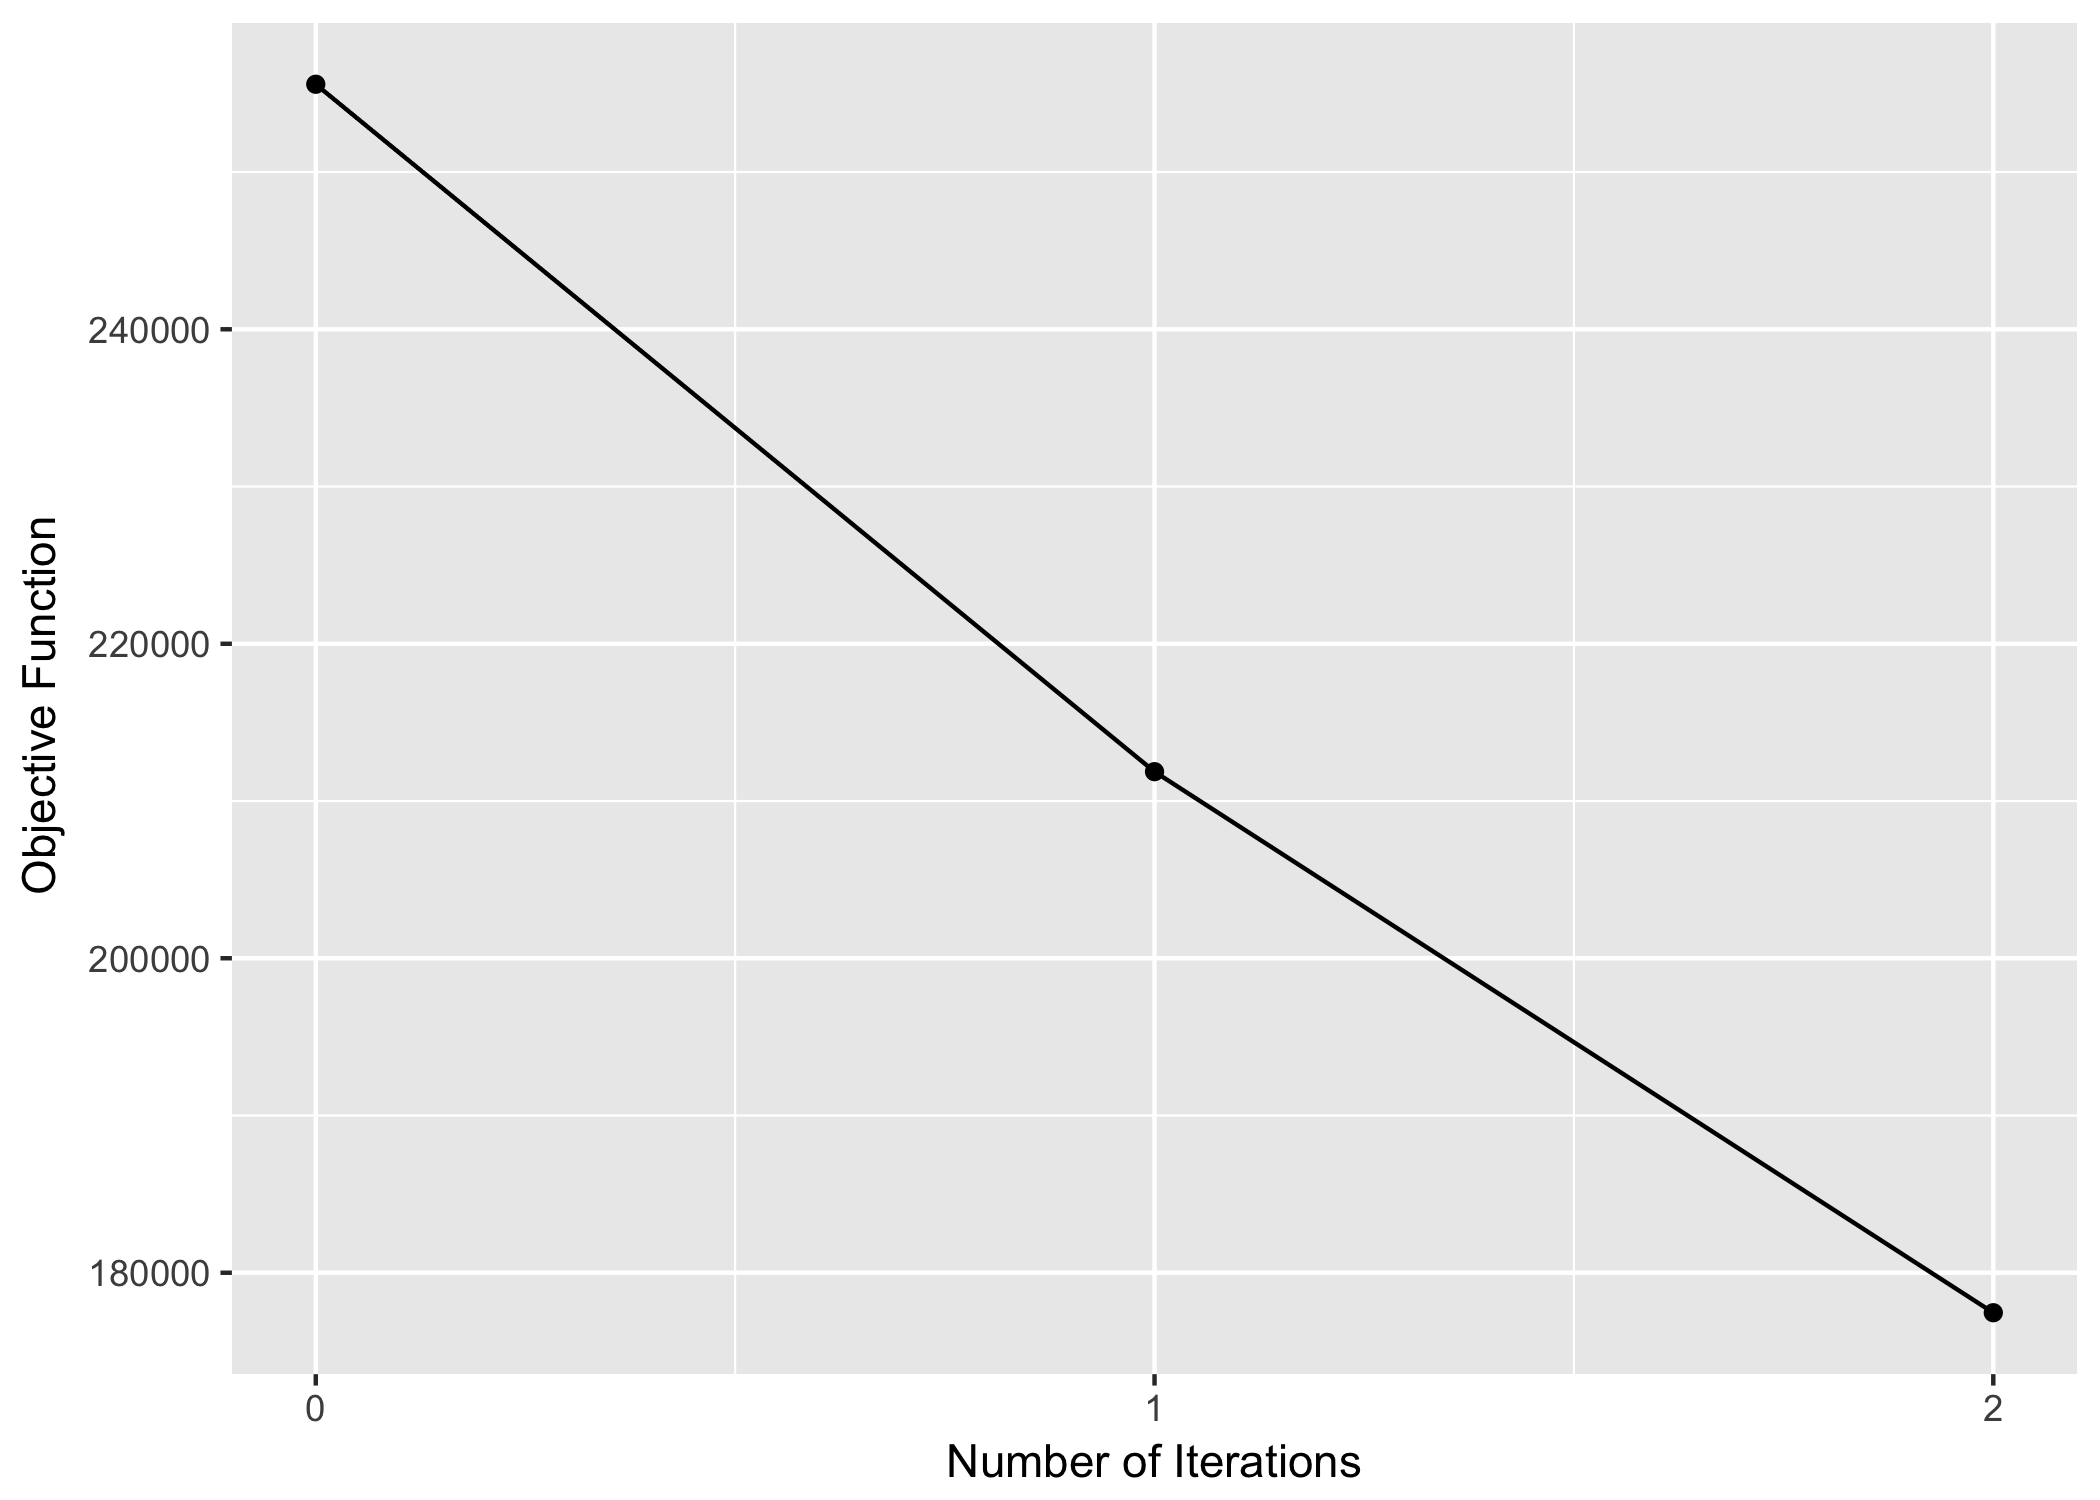
\includegraphics[width=6cm,height=6cm]{images_ready/GFO_4_alt.png}

	  	 \end{column}
	  	 \hspace{5 mm}
	  	  \begin{column}{0.5\textwidth}
	  	  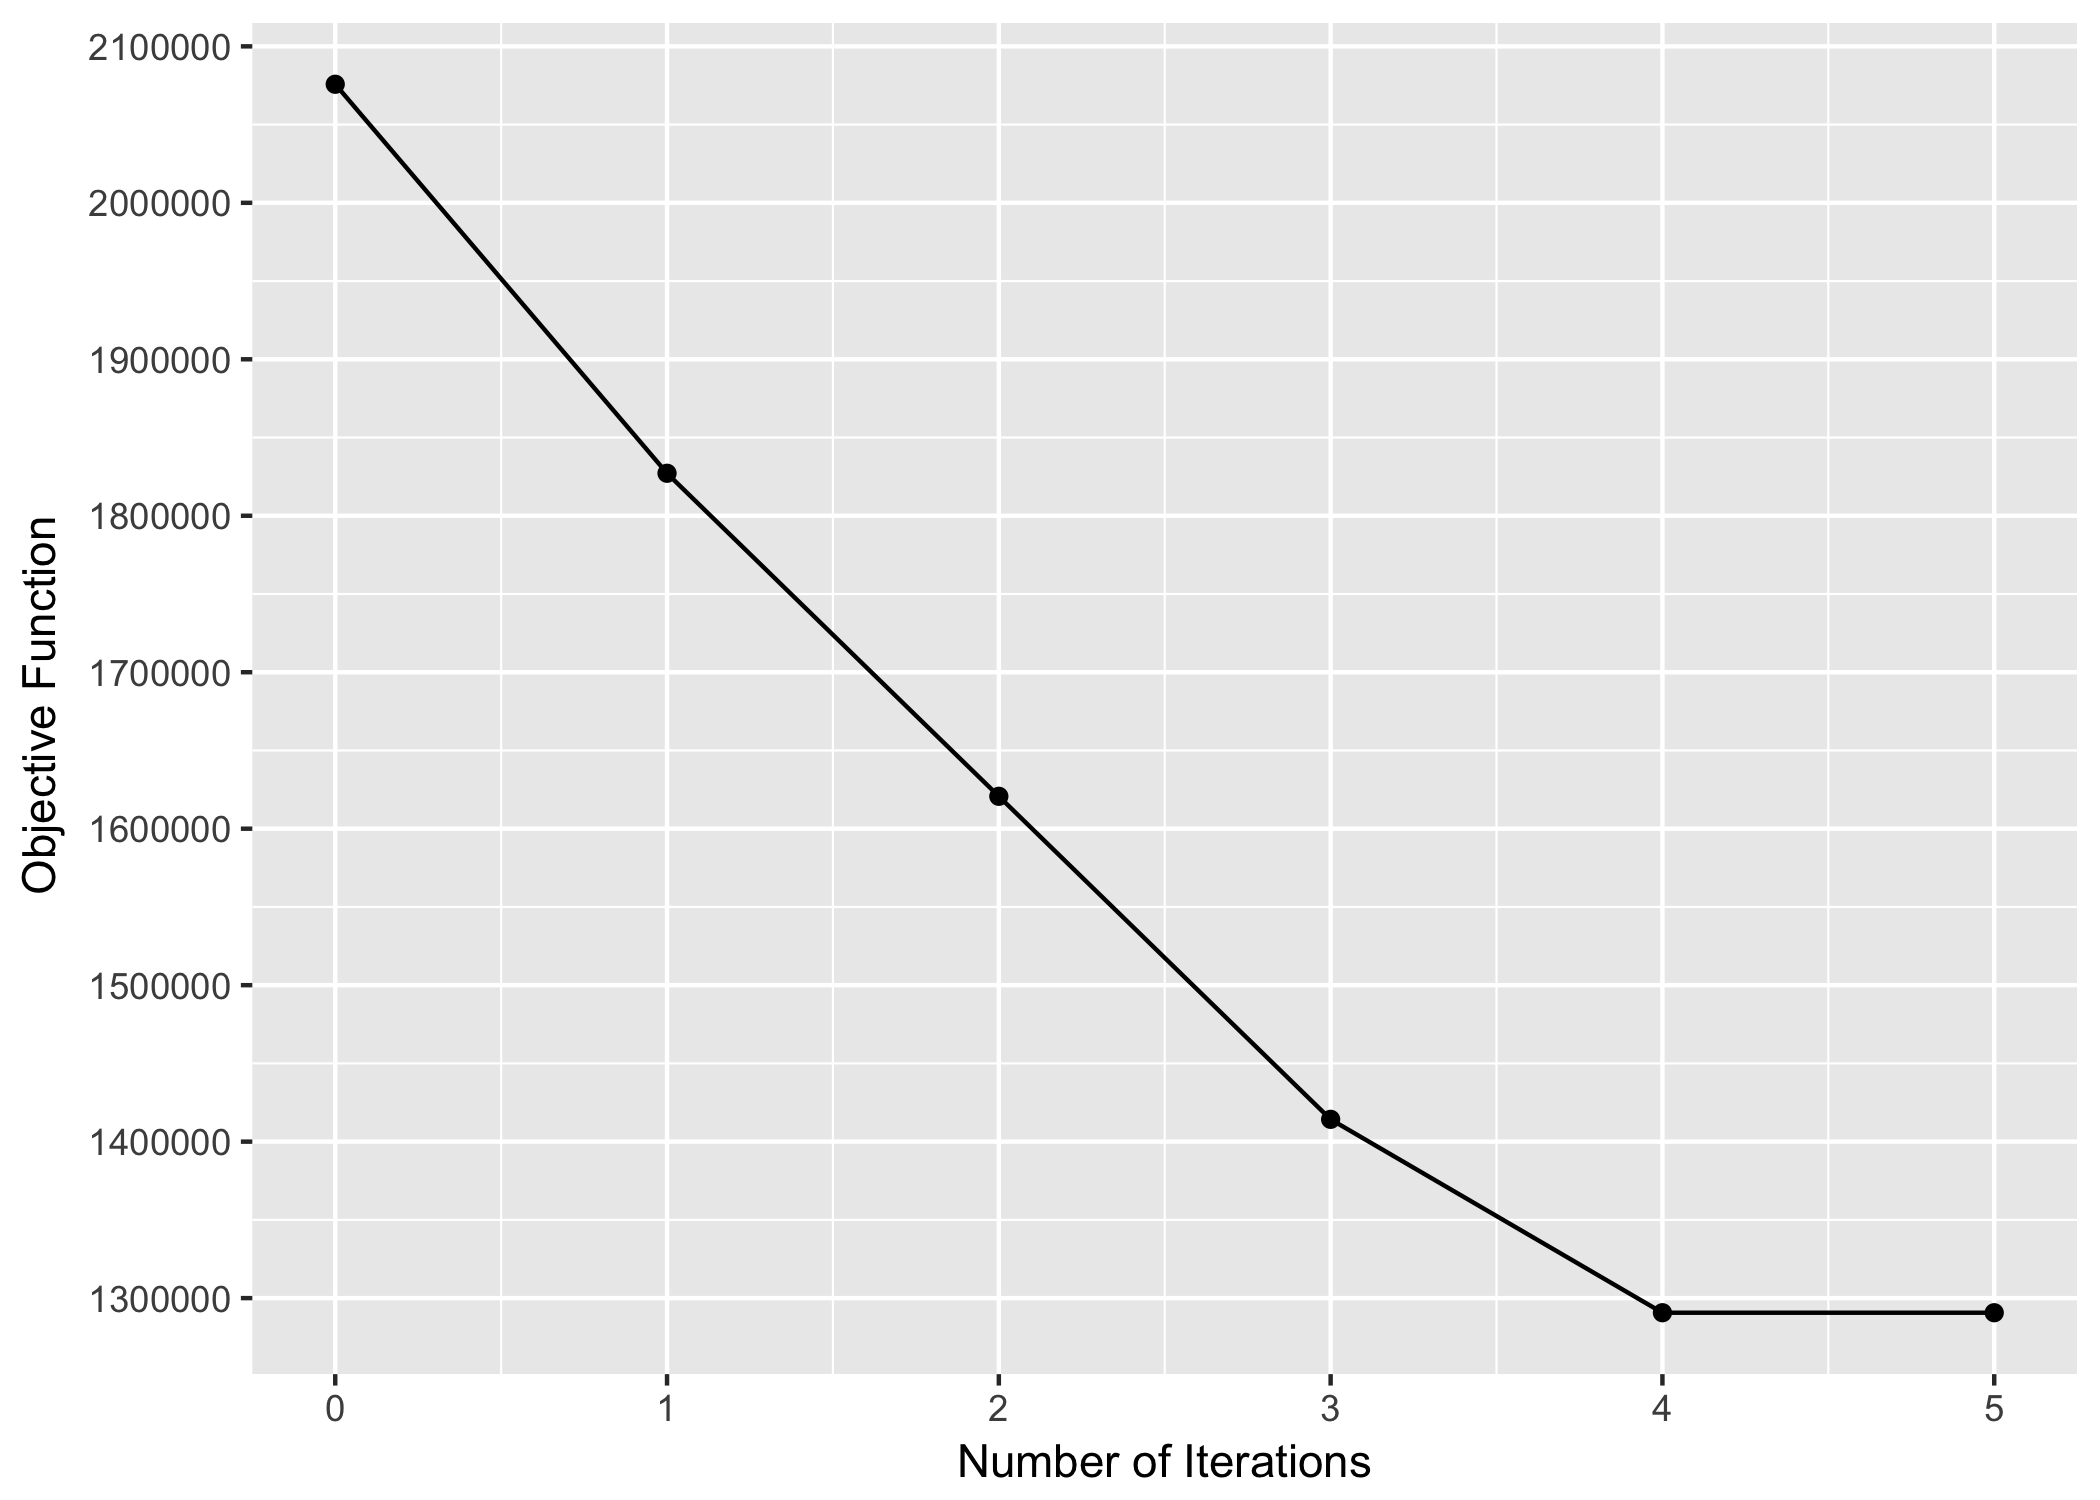
\includegraphics[width=6cm,height=6cm]{images_ready/GFO_8_alt.png}
	  	  	
	  	  \end{column}
	  \end{columns}
	
\end{frame}


\begin{frame}[fragile]
	\frametitle{TEST OBJECTIVE FUNCTION - SEPARING}
	
	\begin{columns}[onlytextwidth]
		\hspace{-8 mm}
		\begin{column}{0.5\textwidth}
			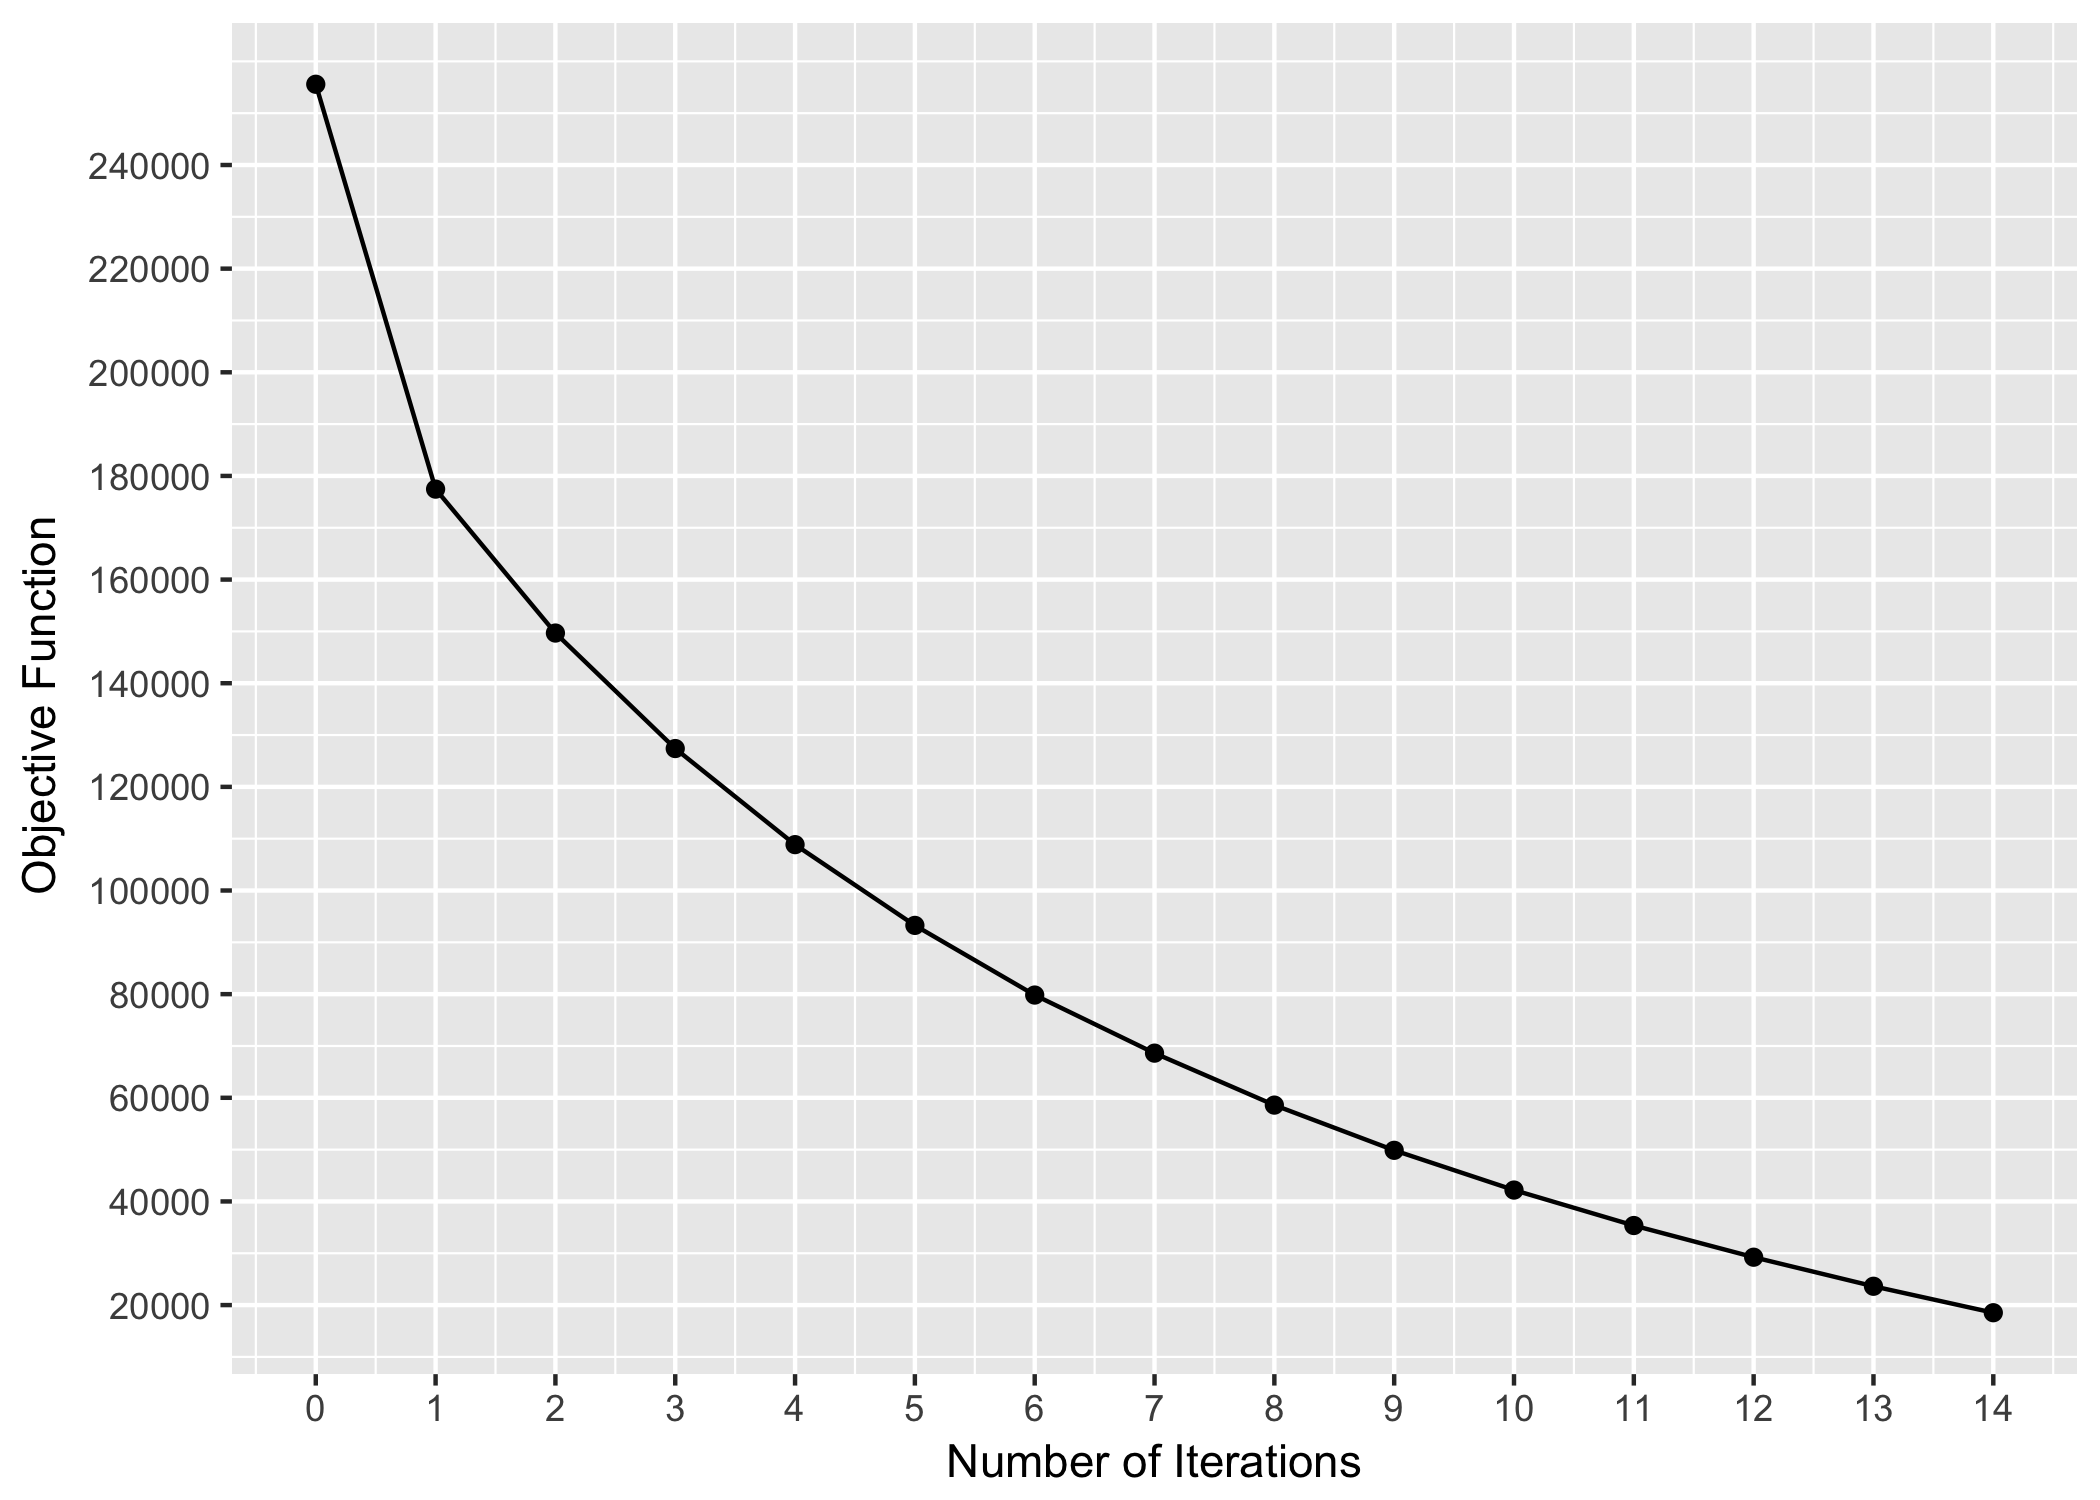
\includegraphics[width=6cm,height=6cm]{images_ready/GFO_4_sep.png}
			
		\end{column}
		\hspace{5 mm}
		\begin{column}{0.5\textwidth}
			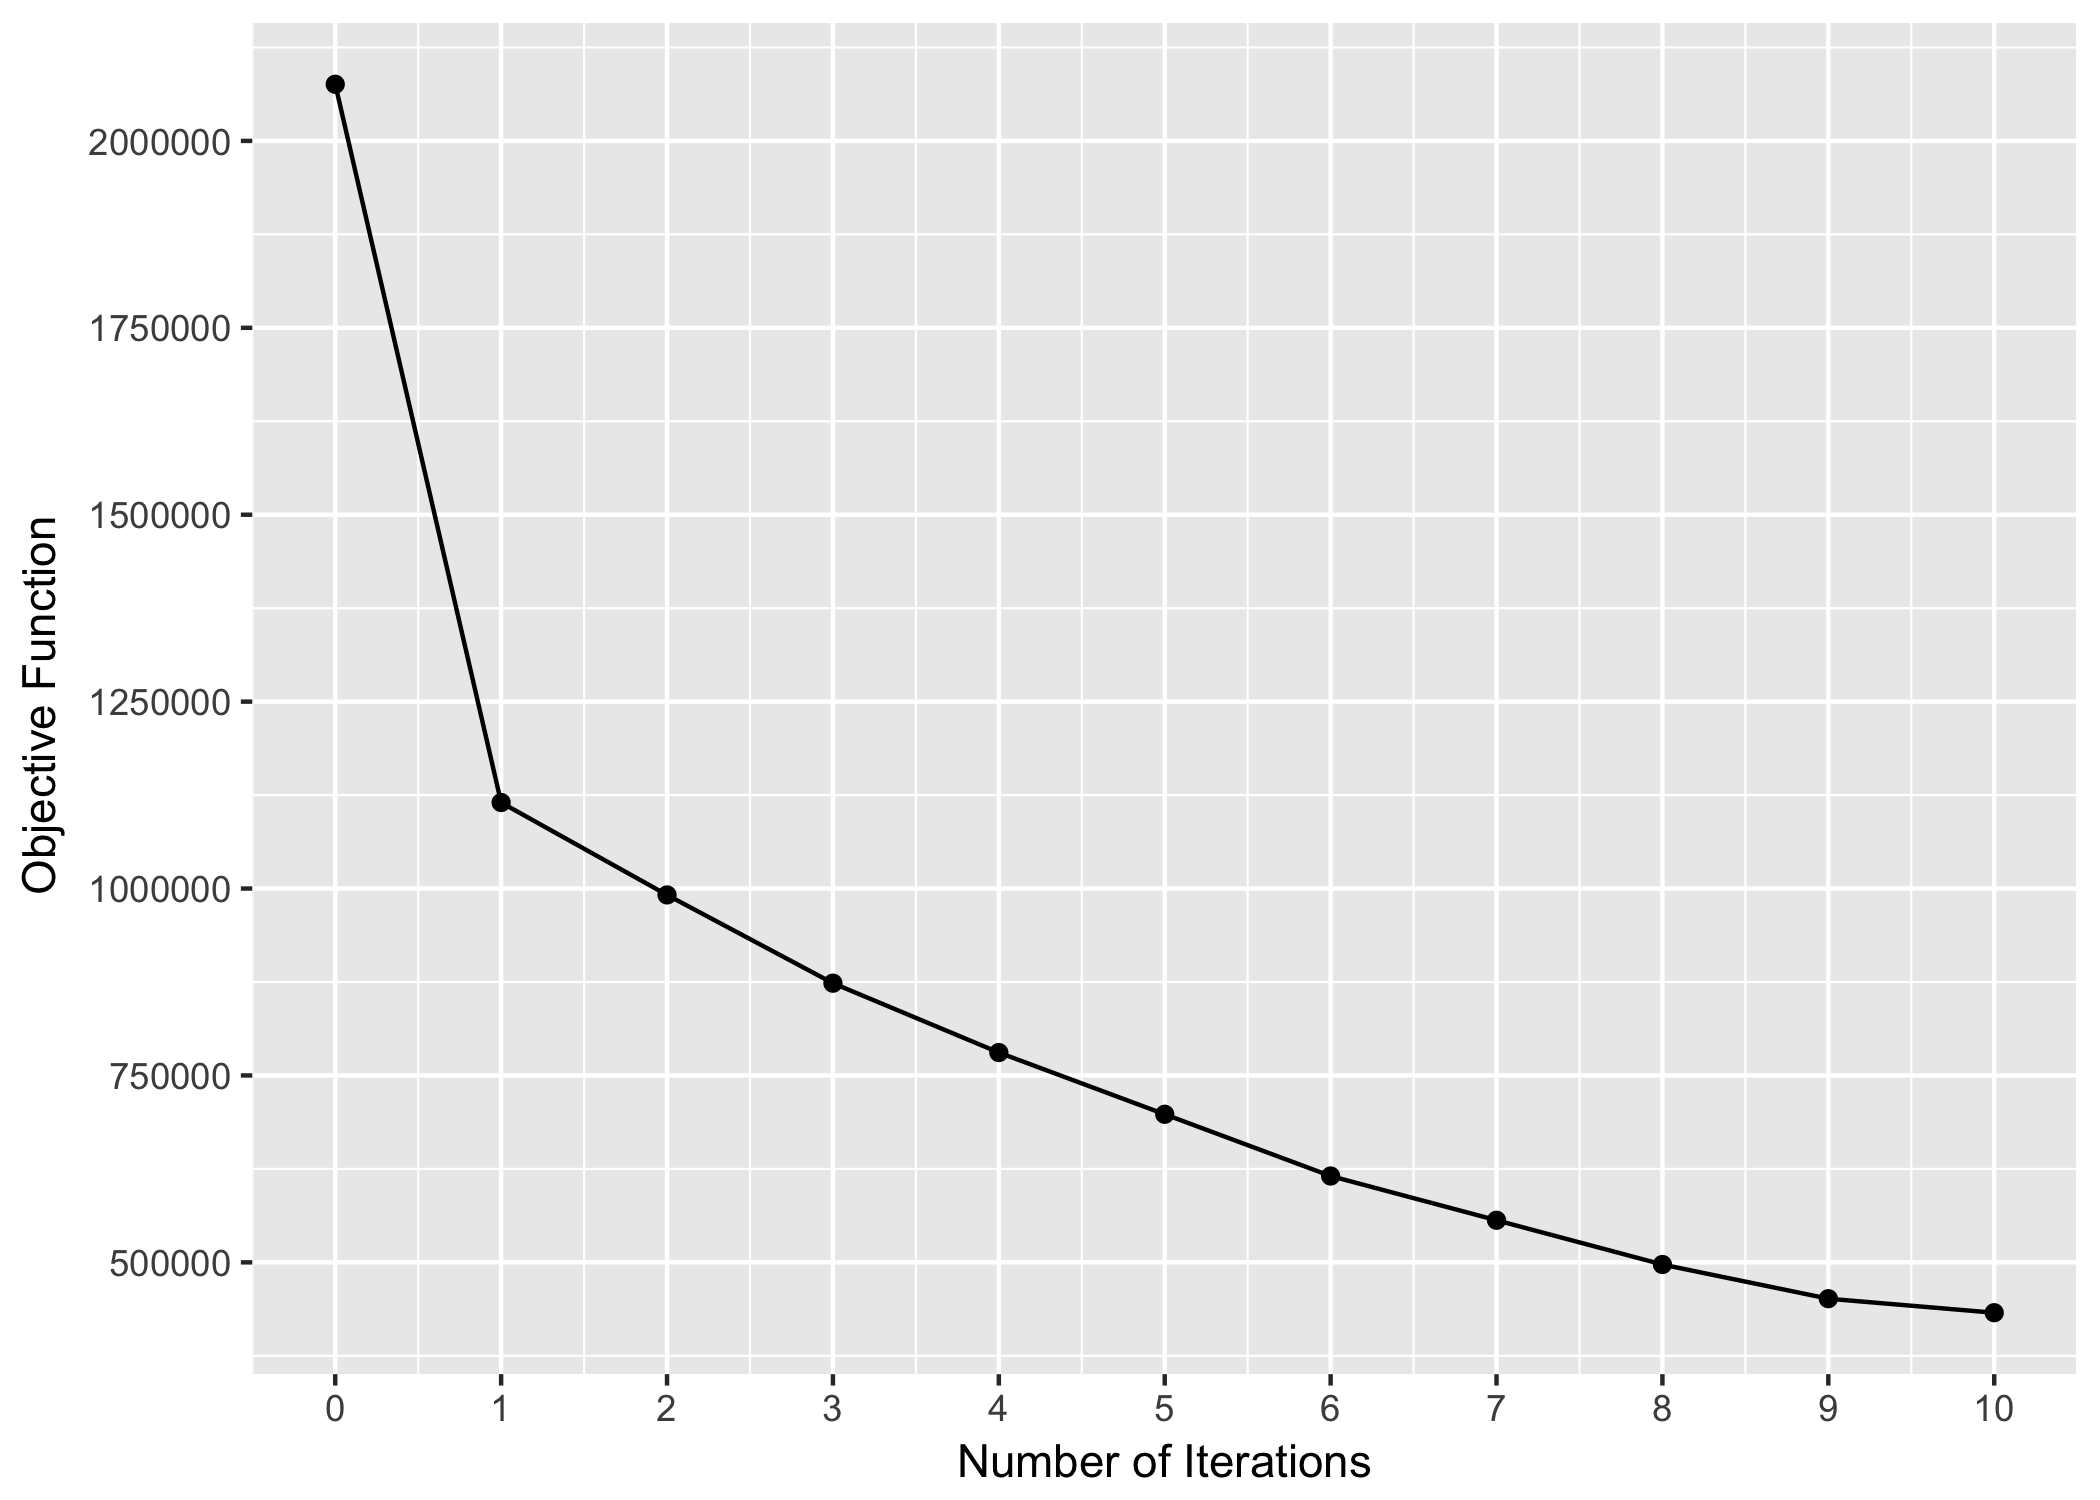
\includegraphics[width=6cm,height=6cm]{images_ready/GFO_8_sep.png}
			
		\end{column}
	\end{columns}
	
\end{frame}


\begin{frame}[fragile]
	\frametitle{TEST TIME PERFORMANCE - ALTERNING}
	
	\textbf{Cache off}
	\begin{columns}[onlytextwidth]
		\hspace{-10 mm}
		\begin{column}{0.5\textwidth}
			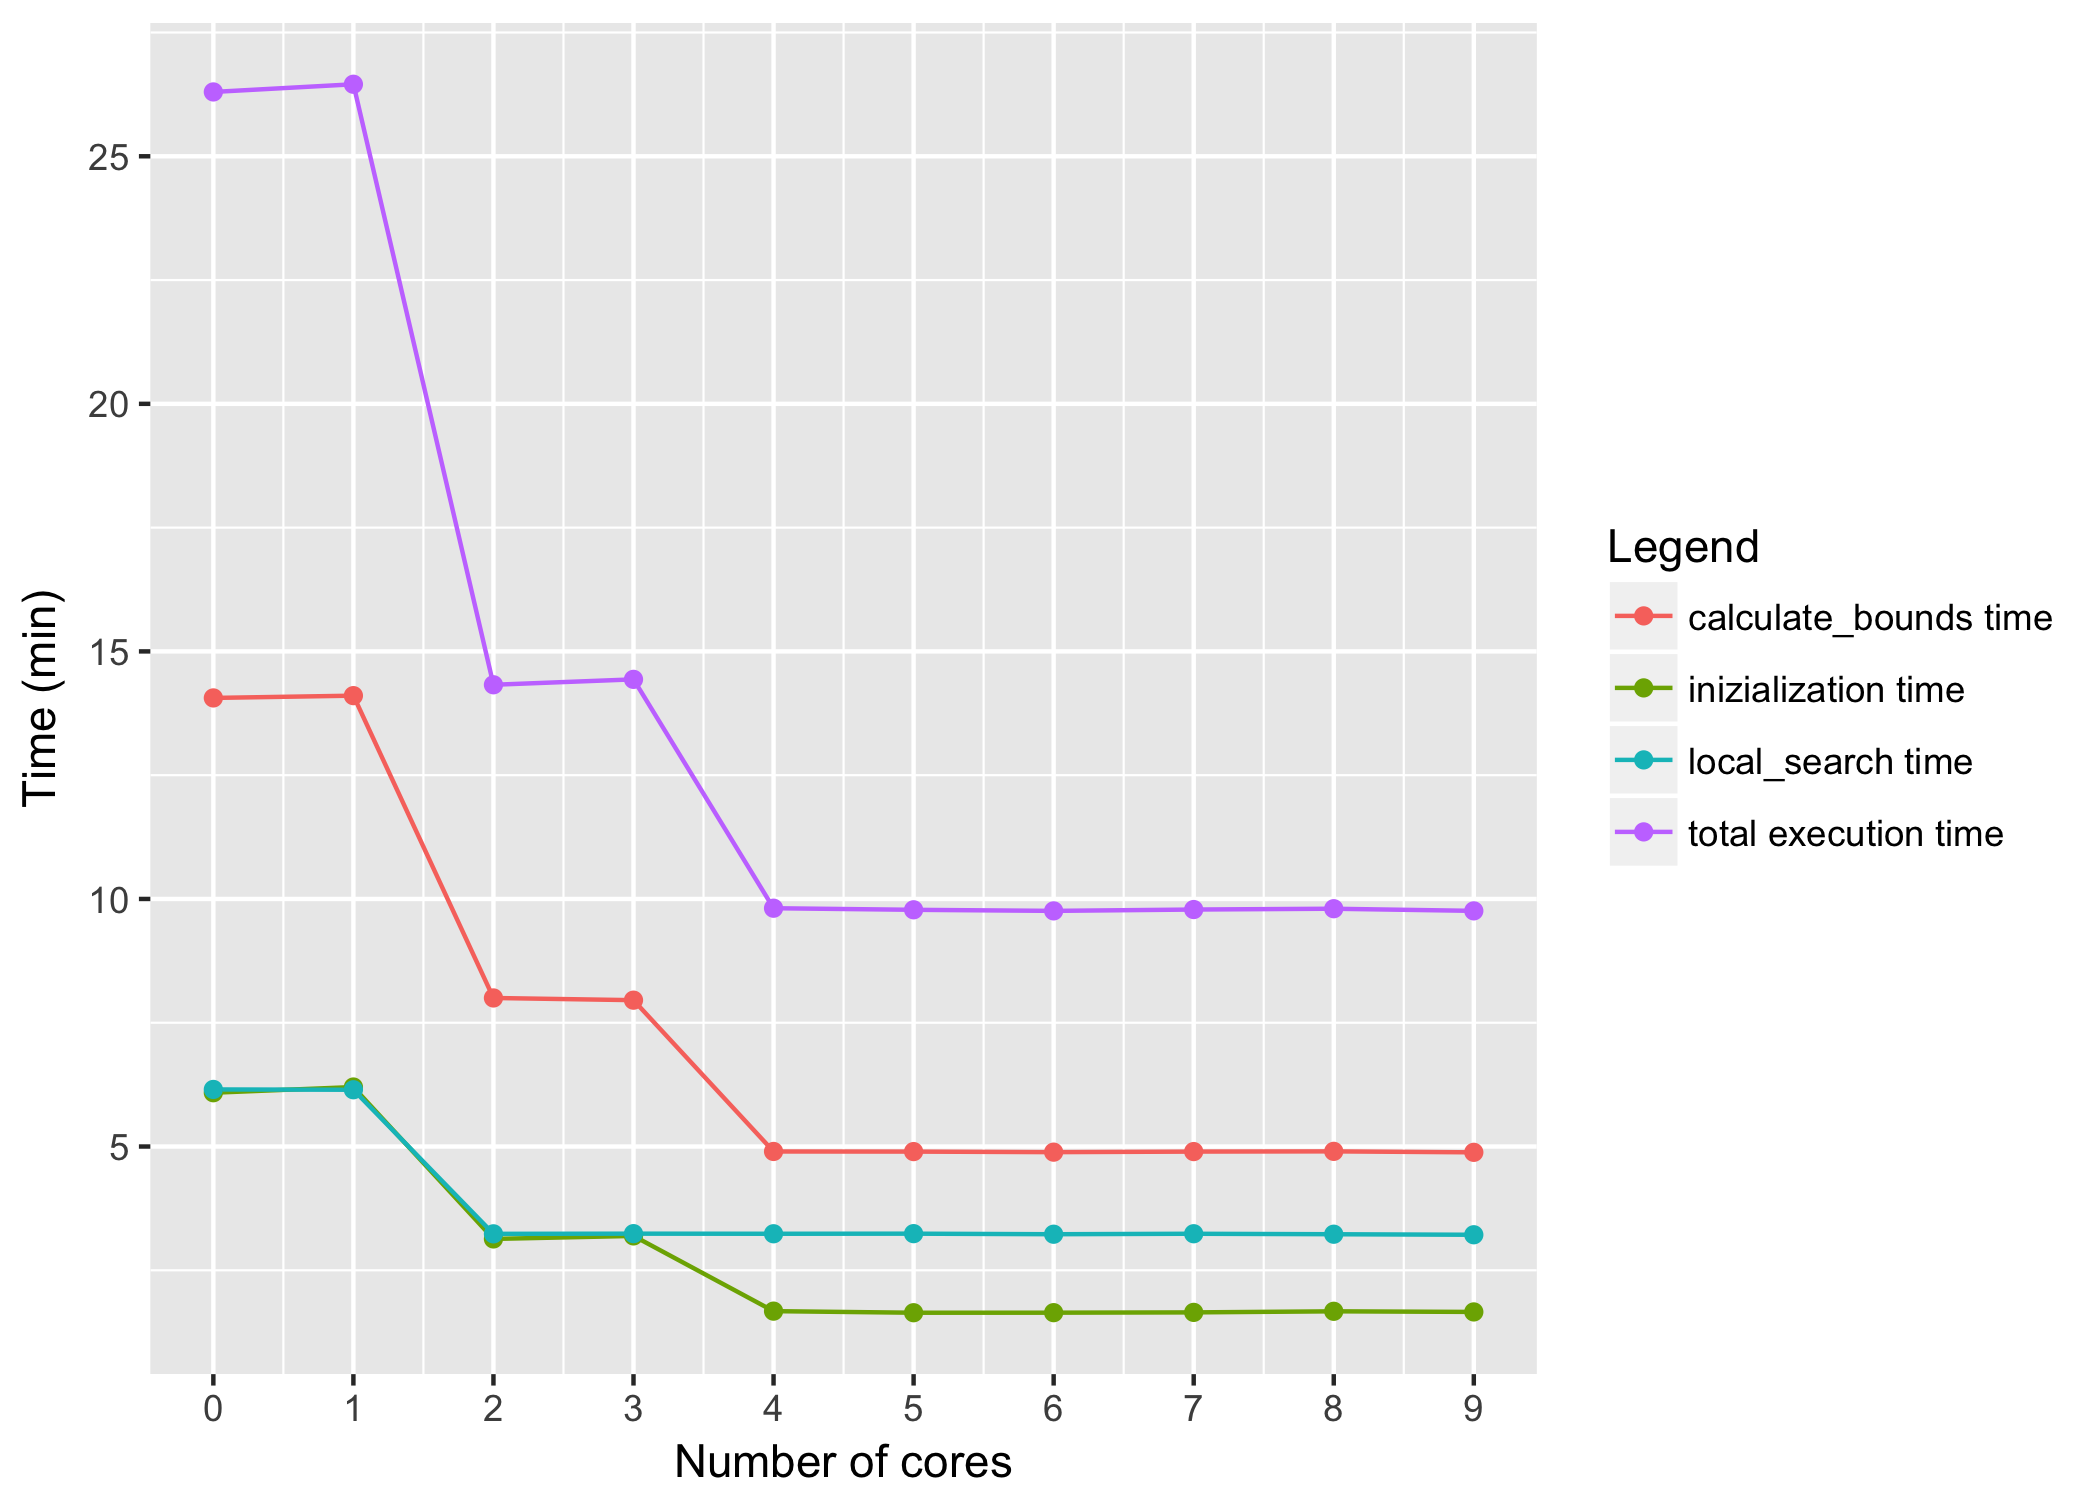
\includegraphics[width=6.3cm,height=6cm]{images_ready/test1_150_10_0_no_a.png}
			
		\end{column}
		\hspace{3 mm}
		\begin{column}{0.5\textwidth}
			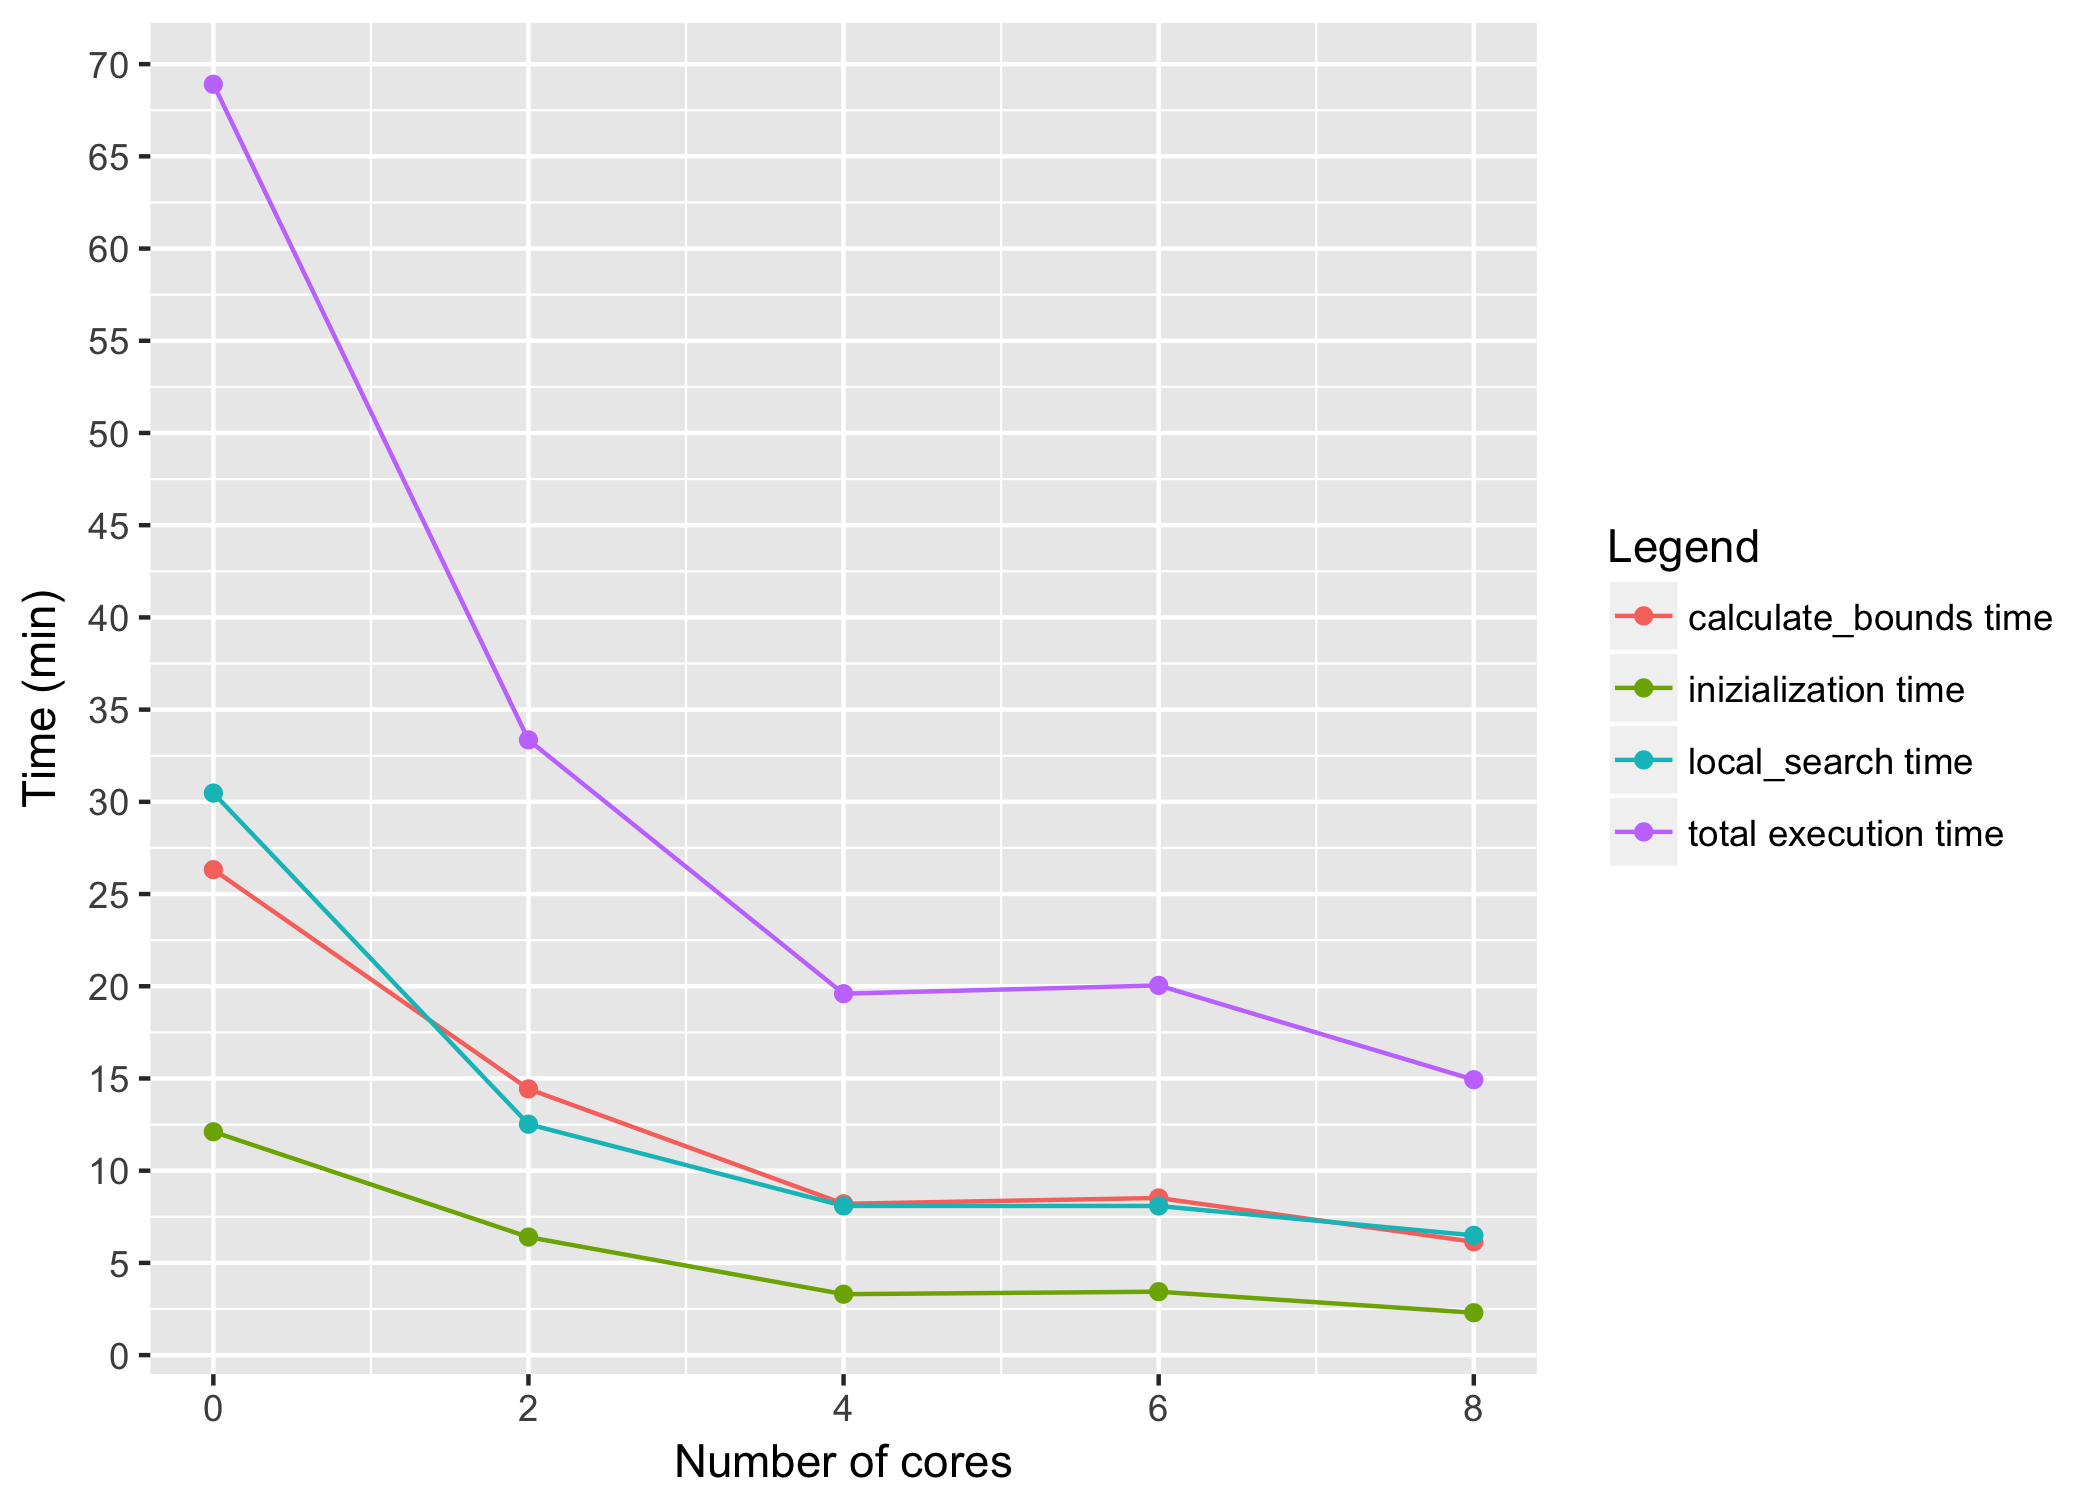
\includegraphics[width=6.3cm,height=6cm]{images_ready/test9_150_10_0_no_a.png}
			
		\end{column}
	\end{columns}
	Even starting from an empty cache this scenario is pessimistic, since there are probably some repetitions in invoking dagSim.
	
	Nevertheless time measurements are acceptable.
	
\end{frame}

\begin{frame}[fragile]
	\frametitle{TEST TIME PERFORMANCE - ALTERNING}
	A realistic scenario: \textbf{50\% cache}
	
	\hspace{22 mm}
	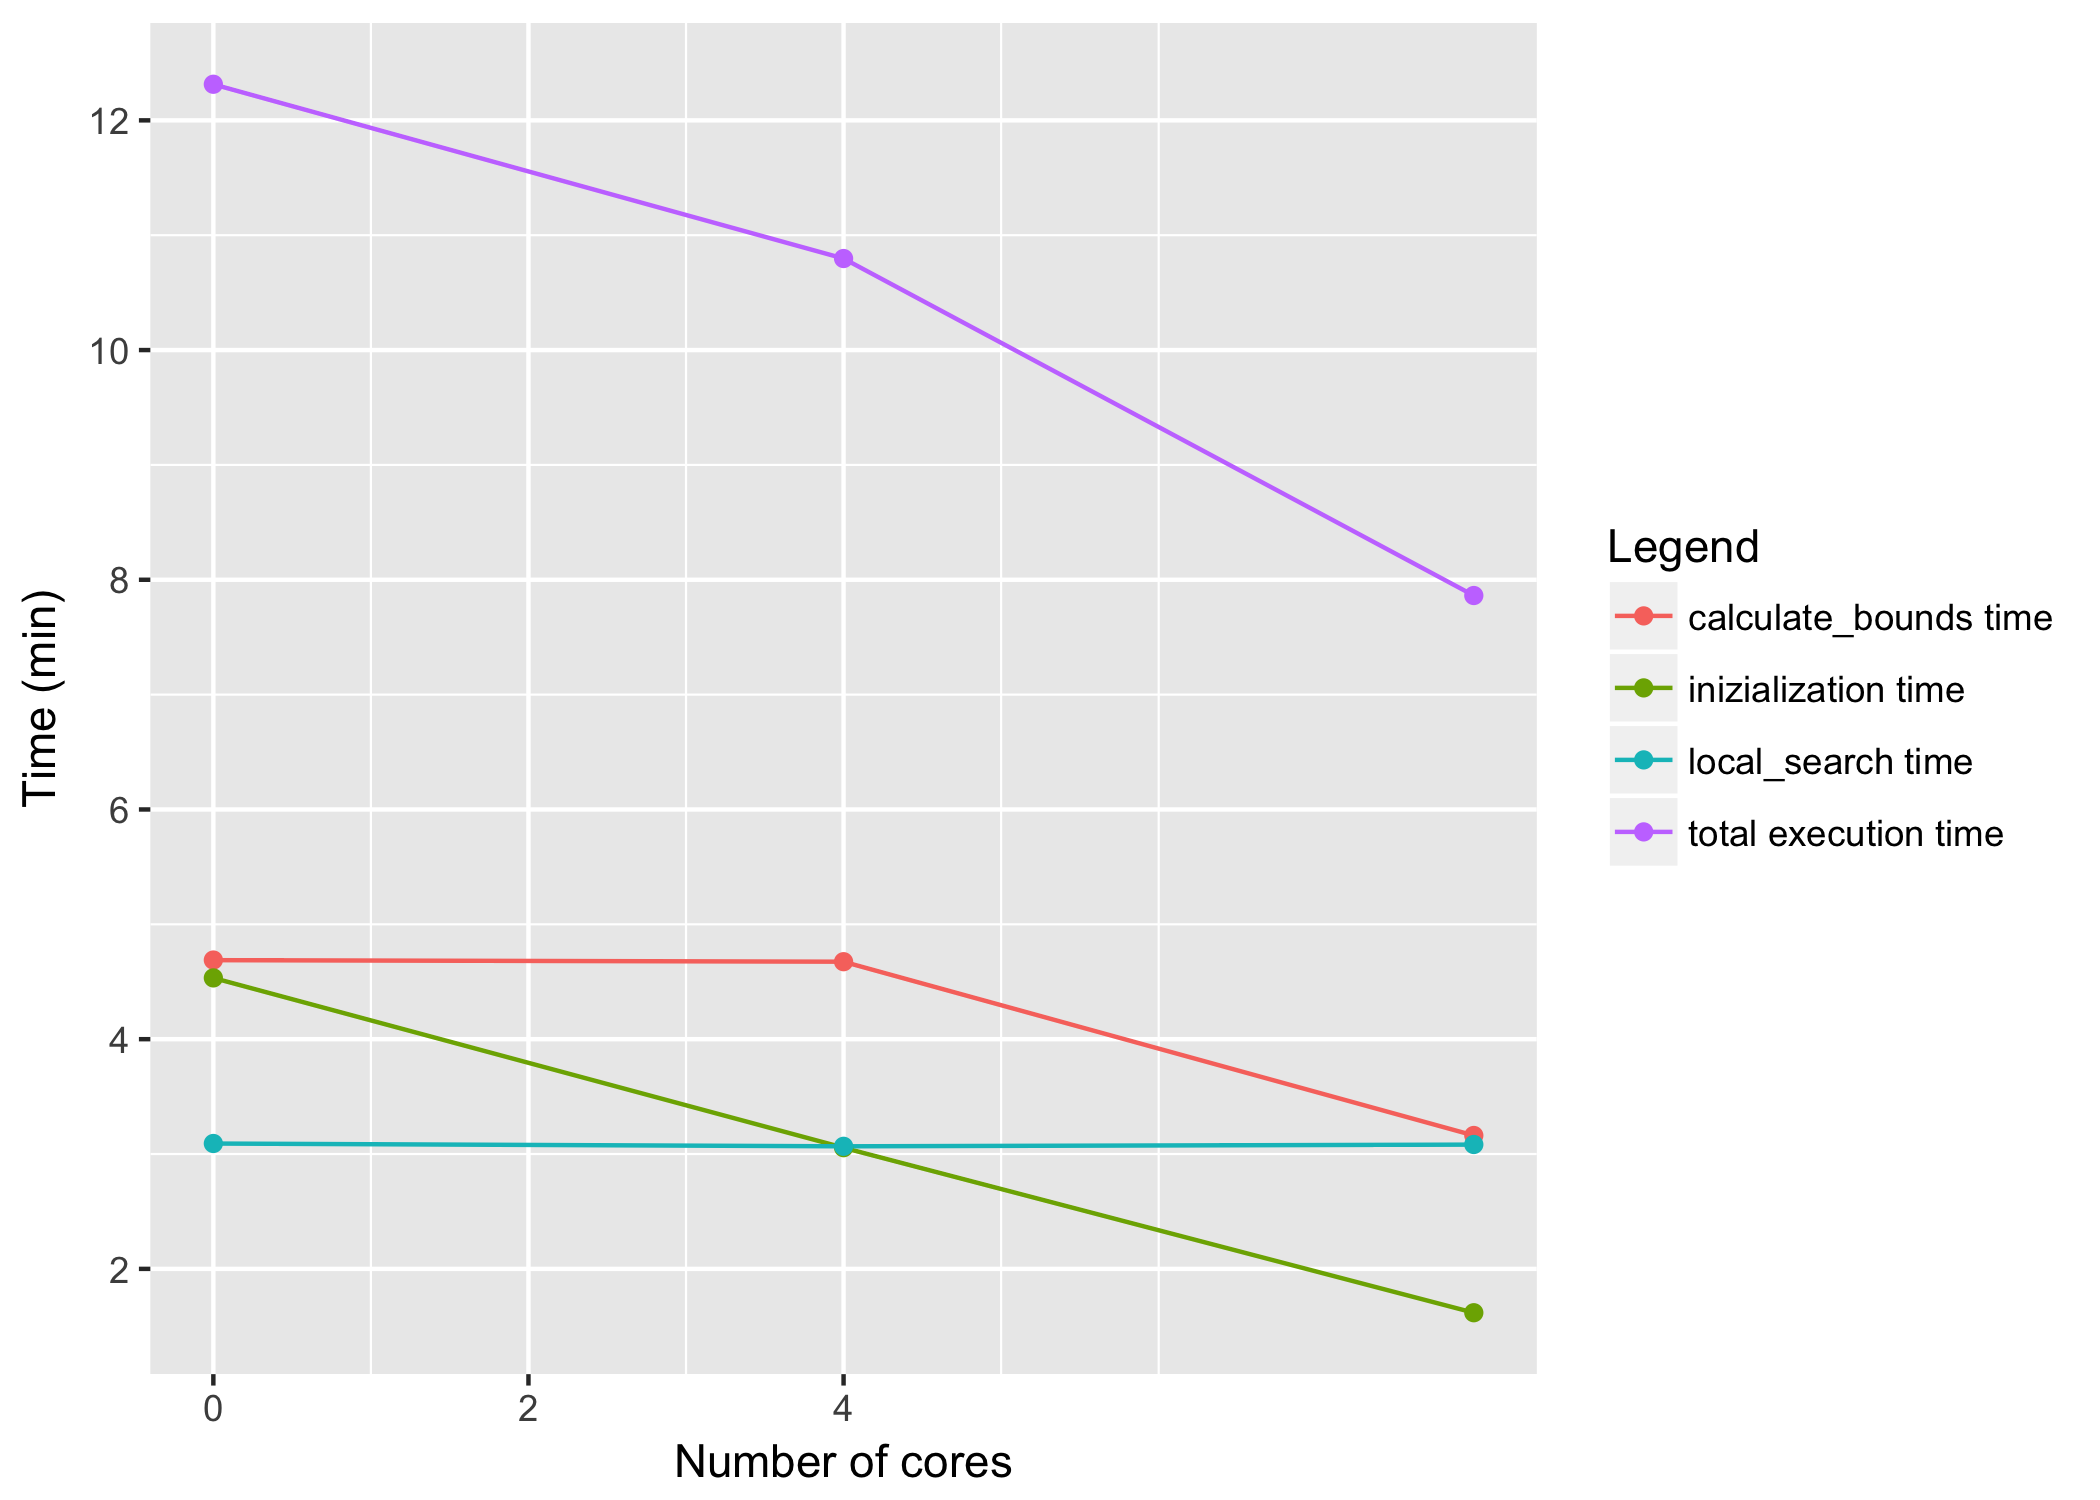
\includegraphics[width=6.3cm,height=5cm]{images_ready/test1_150_10_0_50pc_a.png}

\end{frame}

\begin{frame}[fragile]
	\frametitle{TEST TIME PERFORMANCE - SEPARING}
	
	Many repetitions$\Rightarrow$ very long times with cache off ($\simeq$ 41 minutes with 4 cores and 4 applications)
	
	To represent the worst scenario is more meaningful to turn on the cache and start from an empty database.
	
	\textbf{0\% cache}
	
	\hspace{22 mm}
	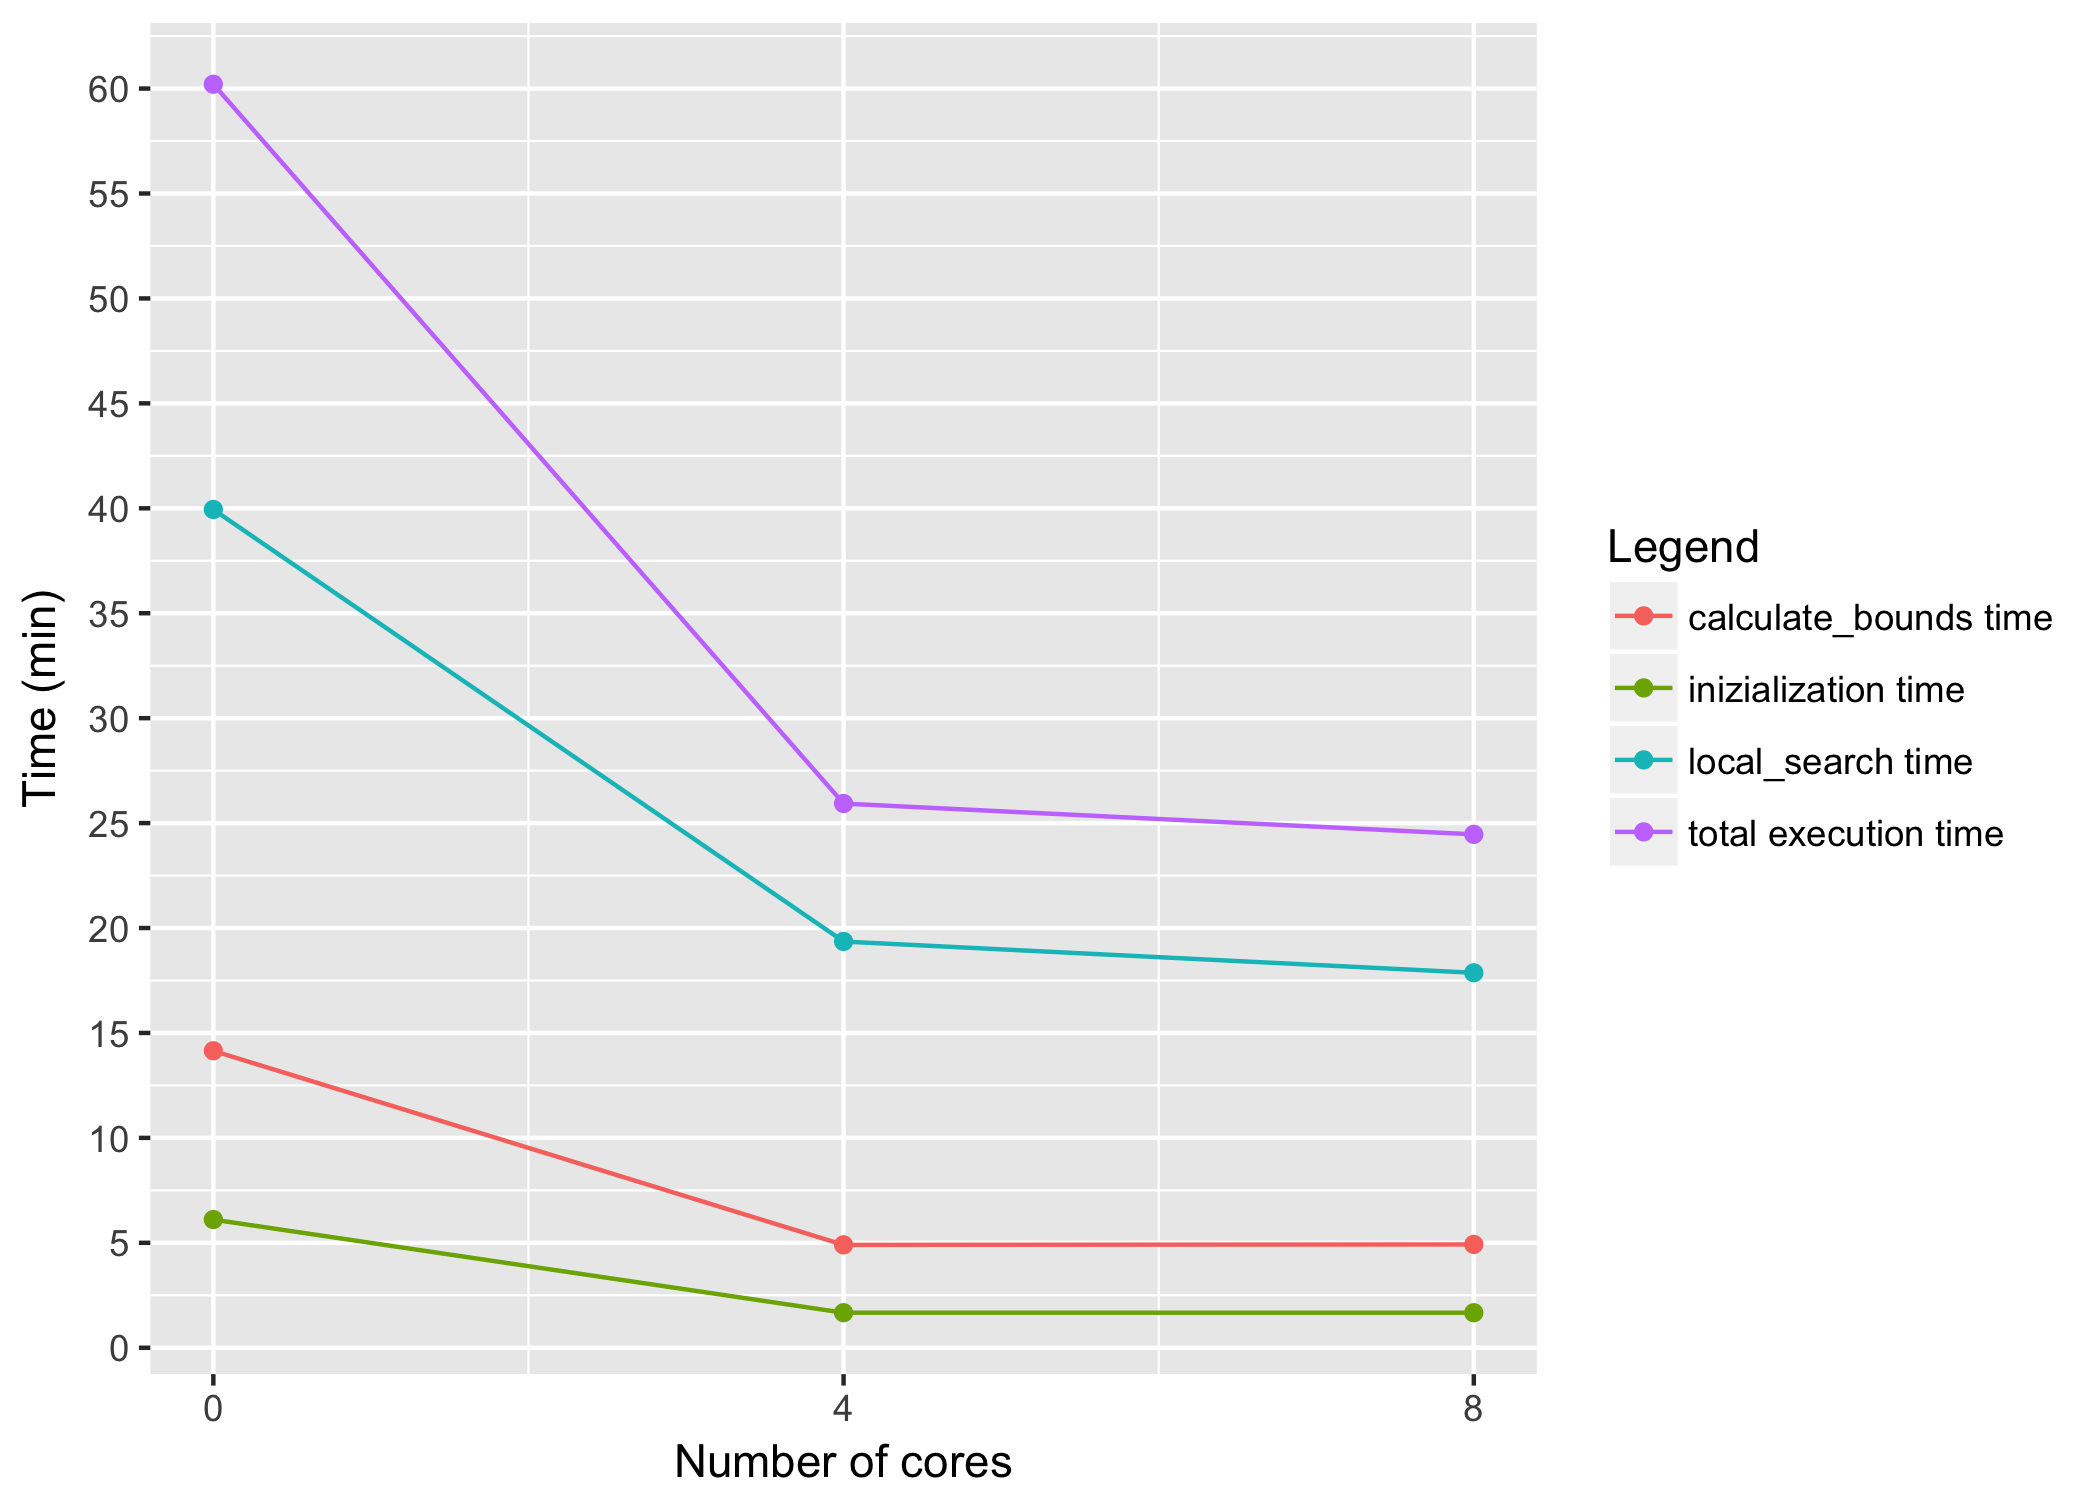
\includegraphics[width=6.3cm,height=5cm]{images_ready/test1_150_10_0_0pc_s.png}
	
	
	
\end{frame}


\begin{frame}[fragile]
	\frametitle{TEST TIME PERFORMANCE - SEPARING}
	A realistic scenario: \textbf{50\% cache}
	
	\hspace{22 mm}
	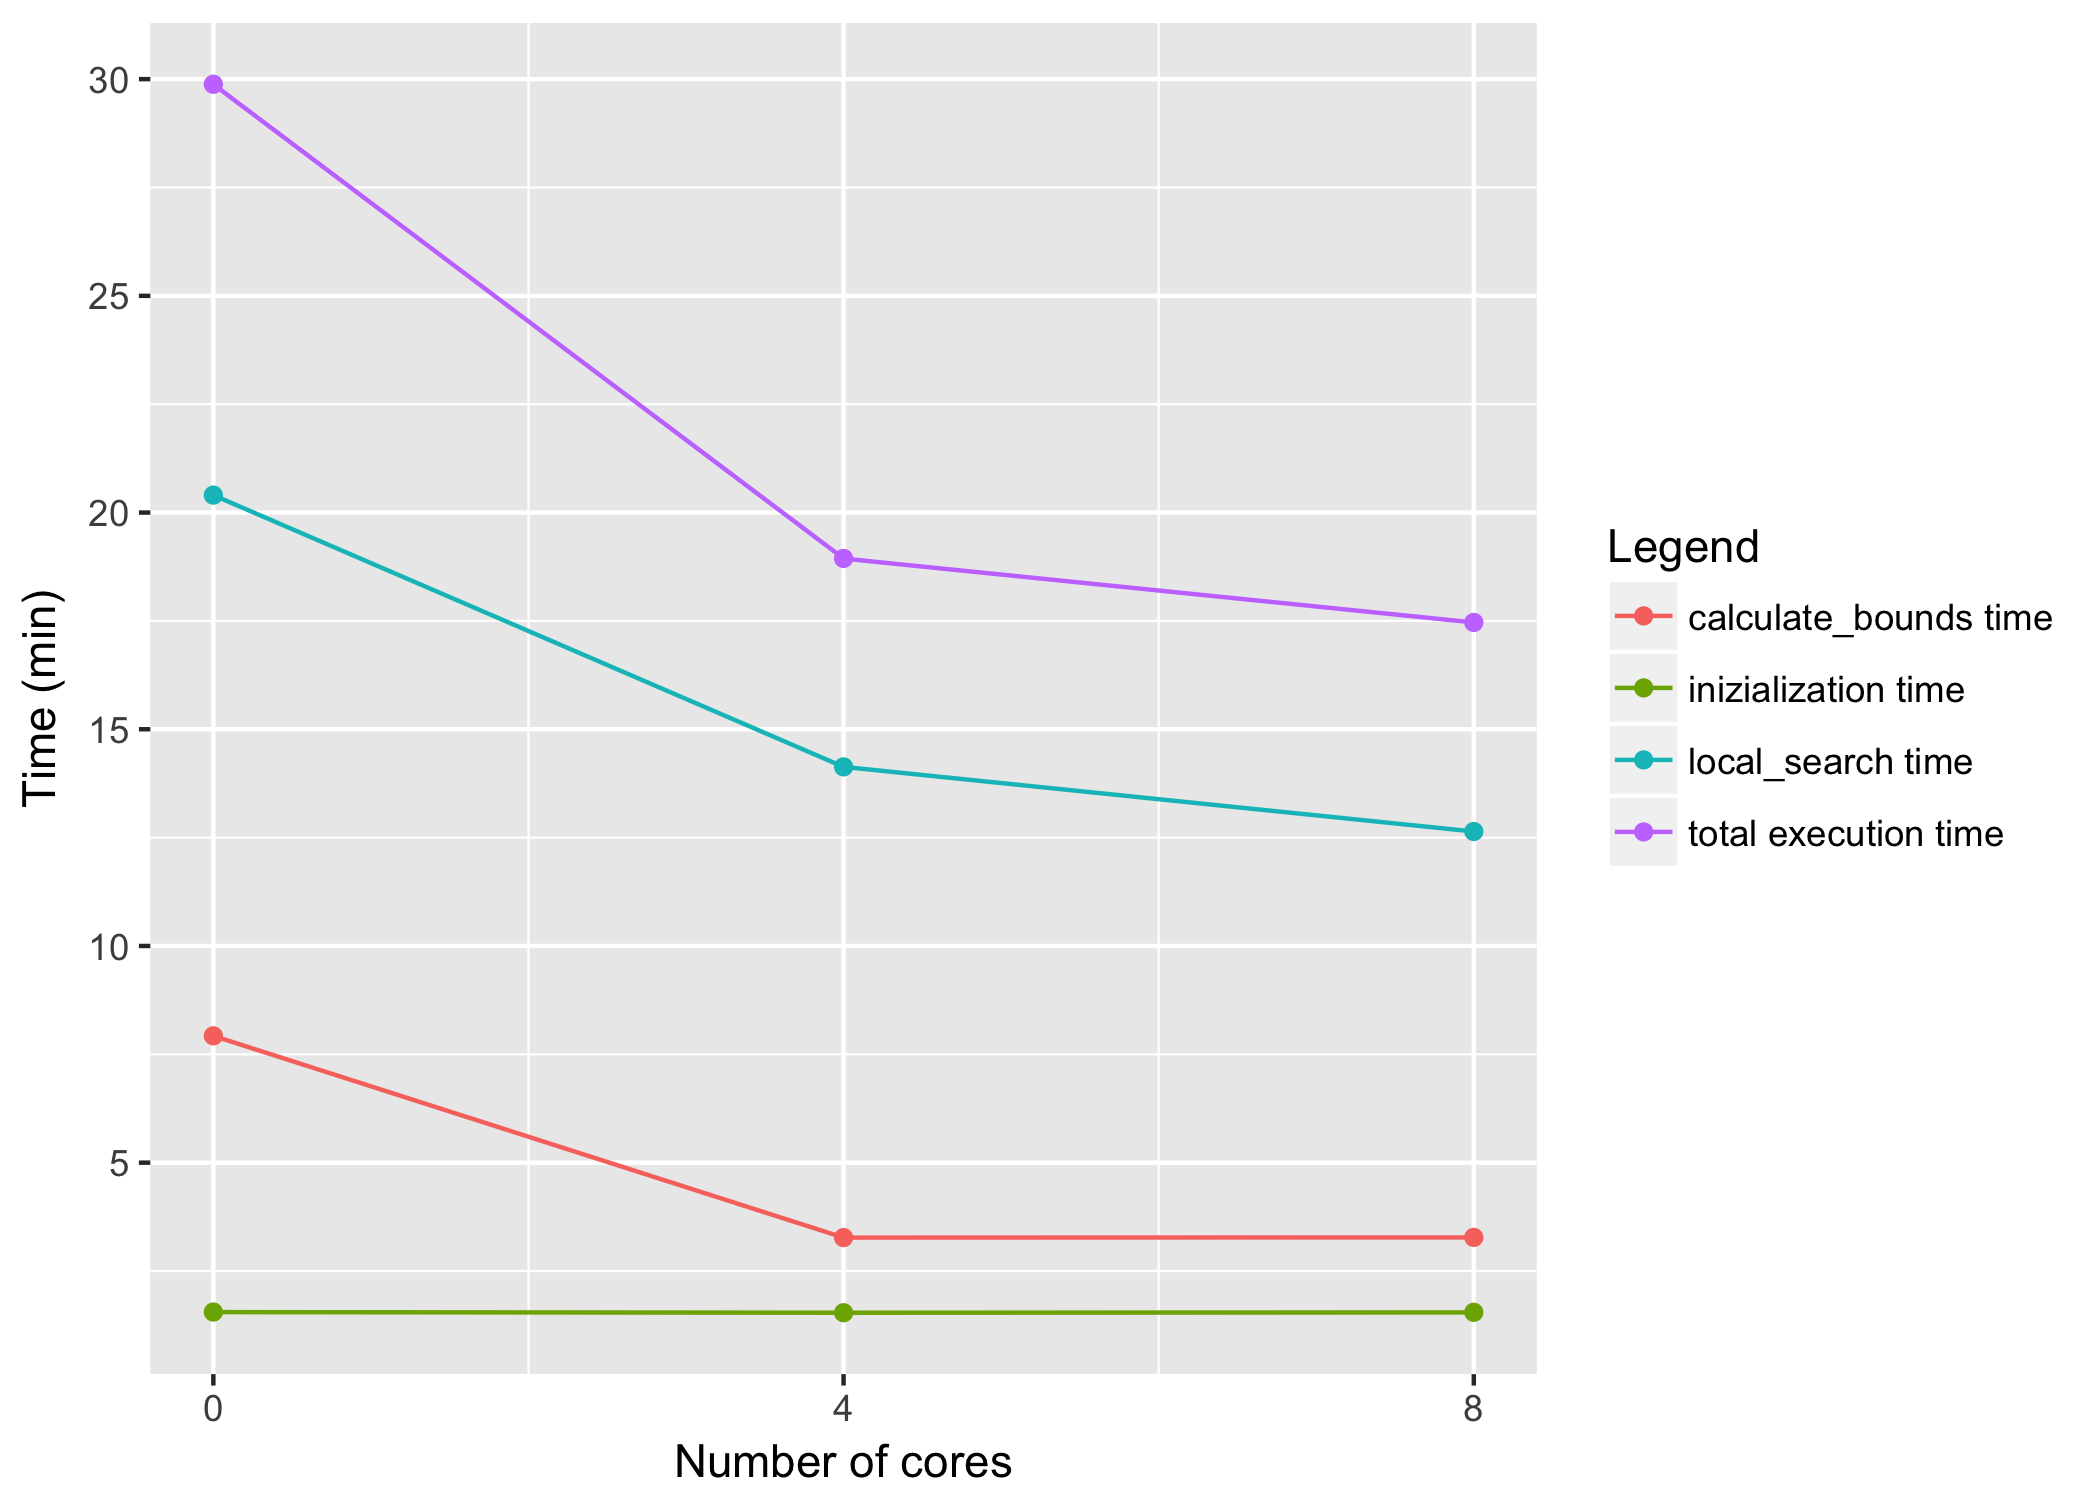
\includegraphics[width=6.3cm,height=5cm]{images_ready/test1_150_10_0_50pc_s.png}
	
	
	
\end{frame}



\begin{frame}[fragile]
	\frametitle{TEST TIME PERFORMANCE - FULL CACHE}
	\centering
	
	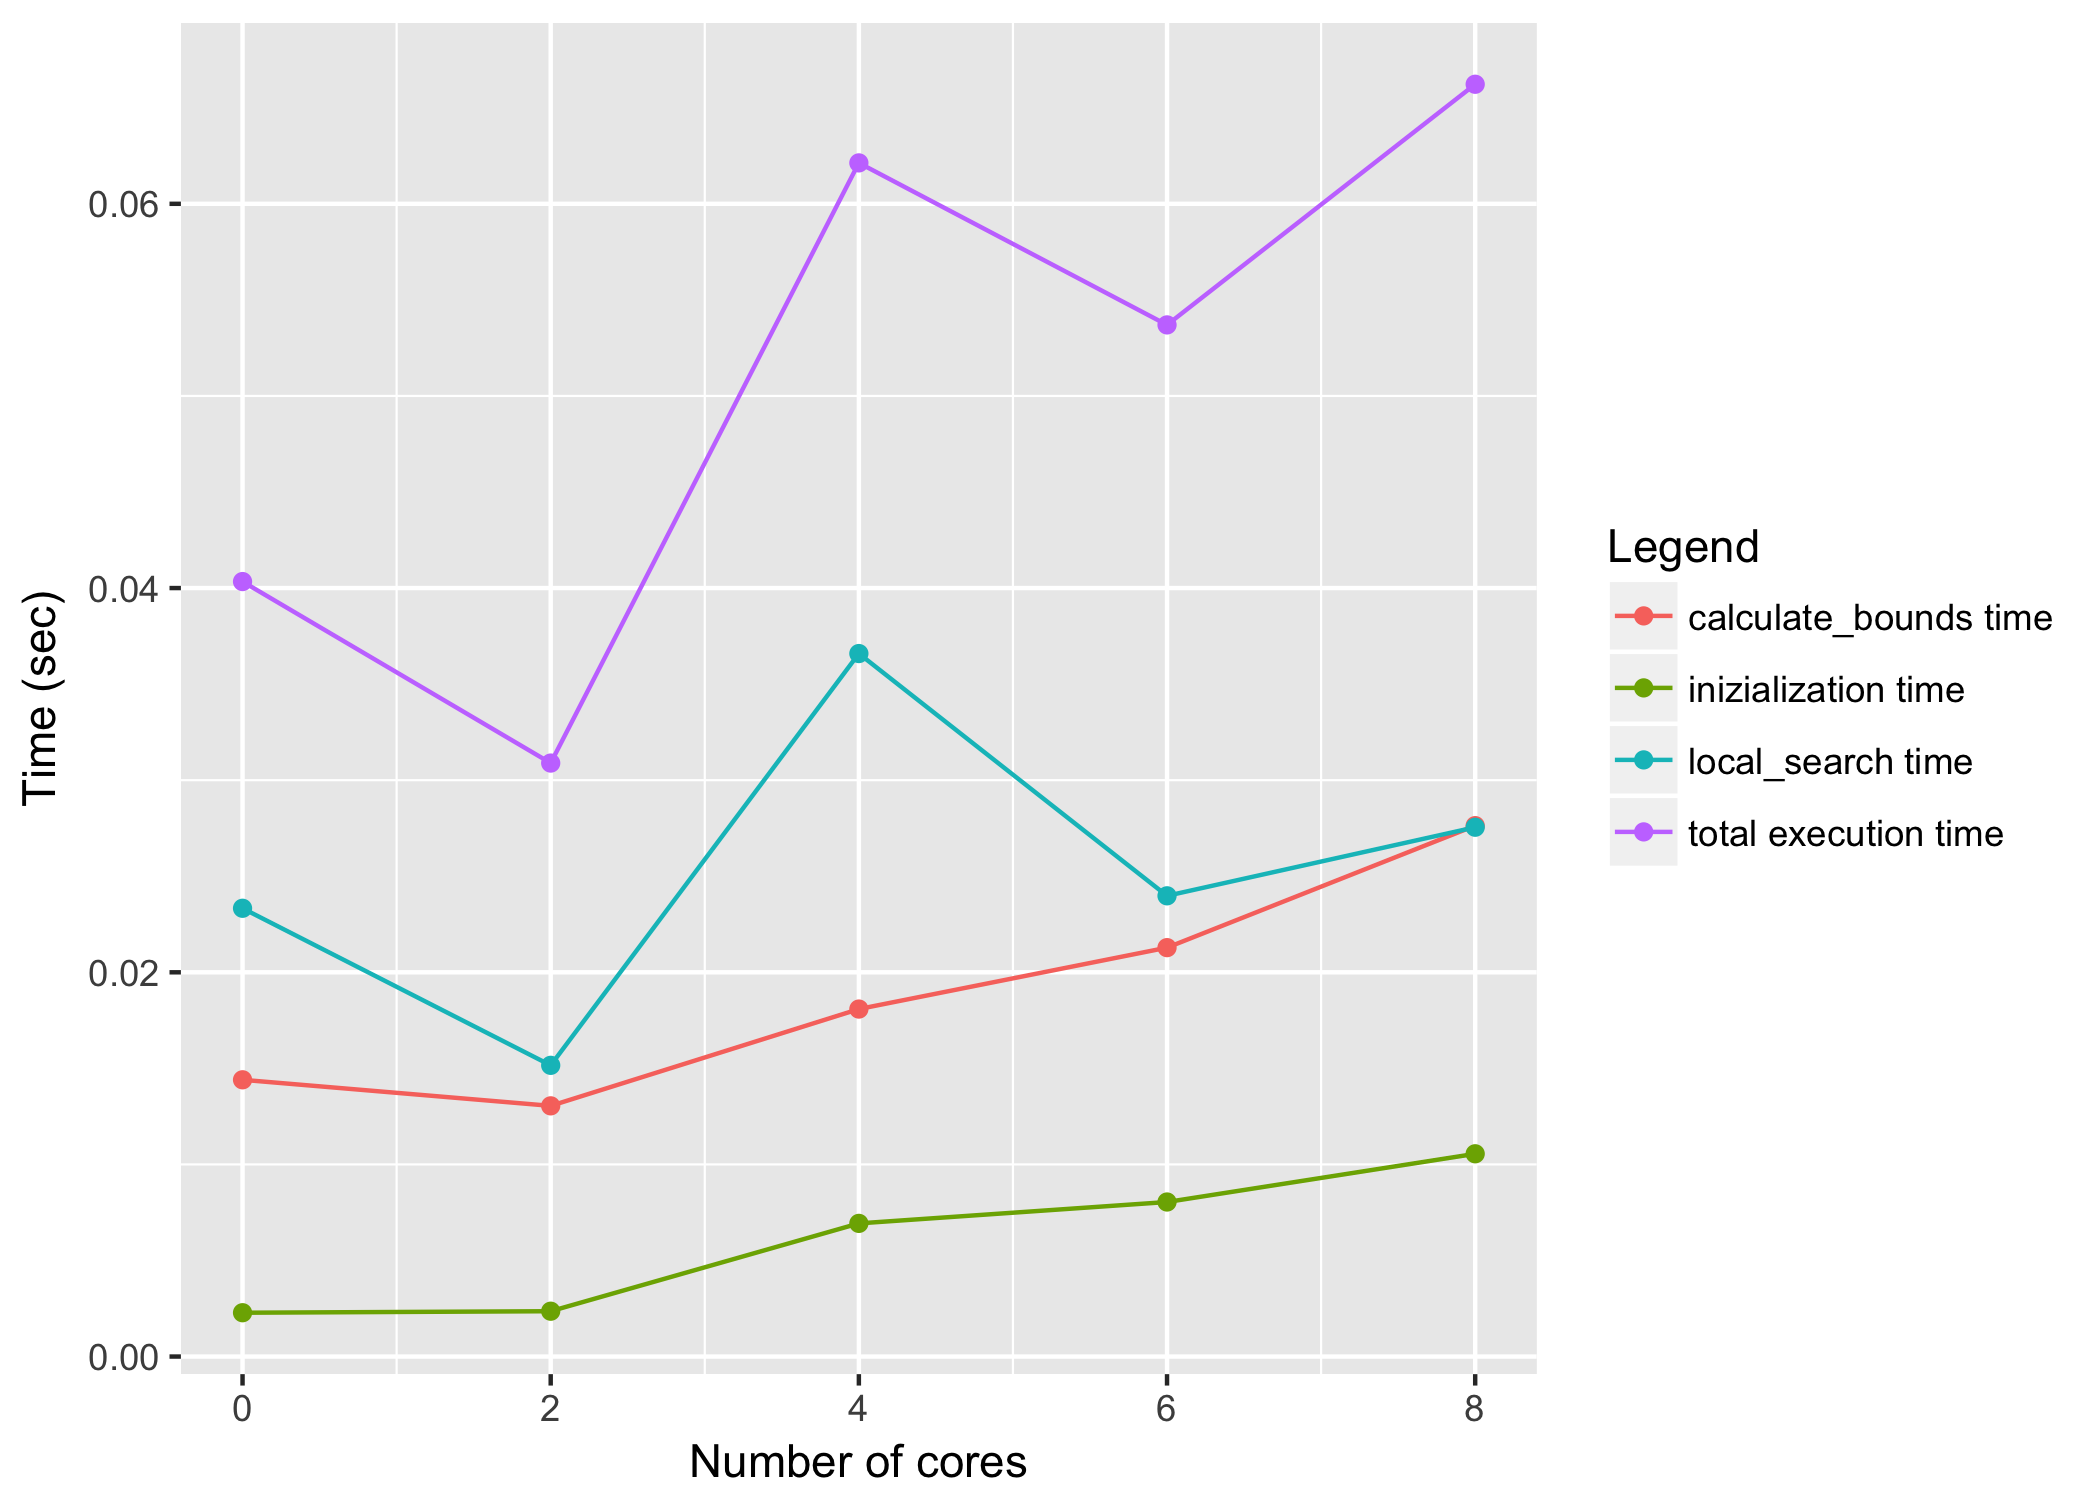
\includegraphics[width=7.3cm,height=6cm]{images_ready/test1_150_10_0_yes_s.png}
			
	
	
\end{frame}










\begin{frame}{BIBLIOGRAPHY}

	\setbeamercolor{item}{fg = black}
  
  \vfill
  References
  \begin{itemize}
  	\item[-] \emph{"D3.2 - Big Data Application Performance models and run-time Optimization Policies", Danilo Ardagna, Enrico Barbierato (Polimi), Jussara M. Almeida, Ana Paula Couto Silva (UFMG)}
  \end{itemize}
  
\end{frame}

\end{document}
